\section{Python}
\begin{frame}{Python}
  \begin{center}
    
\includegraphics[width=140px]{img/python.png} \\
    \color{TUgreen}\textbf{\href{http://python.org}{www.python.org}}
  \end{center}
  \begin{quote}
    \begin{spacing}{1.0}
      Python is a programming language that lets you work more quickly and integrate your systems more effectively. You can learn to use Python and see almost immediate gains in productivity and lower maintenance costs.
    \end{spacing}
  \end{quote}
\end{frame}

\begin{frame}{Python ist...}
  \begin{itemize}
    \item […] eine Programmiersprache.
    \item […] einfach!
    \item […] sehr mächtig.
    \item […] universell einsetzbar.
  \end{itemize}
  \begin{center}
    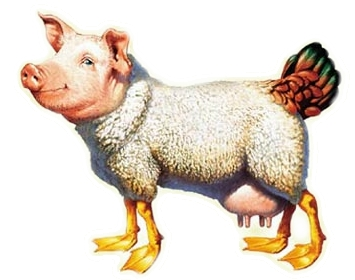
\includegraphics[width=120px]{img/eierlegendewollmilchsau.jpg}\\
    \tiny\texttt{\href{http://xn--sptzlemitsoss-cfb.de/wp-content/uploads/2012/07/eierlegendewollmilchsau.jpg}{http://xn--sptzlemitsoss-cfb.de/wp-content/uploads/2012/07/eierlegendewollmilchsau.jpg}}\normalsize
  \end{center}
\end{frame}

\begin{frame}[fragile]{Ein kleines Beispiel}
  \vspace{-1em}
  \begin{columns}
    \begin{column}{0.5\textwidth}
      \begin{exampleblock}{C++}
        \begin{minted}{c++}
#include <iostream>
using namespace std;
int main(int argc, char *argv[])
{
    cout << "Hello, World!" << endl;
    return 0;
}
        \end{minted}
      \end{exampleblock}
    \end{column}
    \begin{column}{0.5\textwidth}
      \begin{exampleblock}{Python}
        \begin{minted}{python}
print("Hello, World!")
        \end{minted}
      \end{exampleblock}
    \end{column}
  \end{columns}
\end{frame}

\begin{frame}{Python}
  \tableofcontents[sectionstyle=show/hide,
                   subsectionstyle=show/show/hide,
                   subsubsectionstyle=show/show/show]
\end{frame}

\subsection{iPython}
\begin{frame}{iPython}
\end{frame}

\subsection{Syntax}
\begin{frame}{Variablen, Operatoren}
\end{frame}

\begin{frame}[fragile]{\texttt{(), [], \{\}}}
  \begin{itemize}
    \item[\texttt{()}] Tupel
    \item[\texttt{[]}] Liste
    \item[\texttt{\{\}}] Map 
  \end{itemize}
  \vspace{.5em}
  \begin{spacing}{1.0}
    \begin{exampleblock}{Zum Beispiel}
      \begin{minted}{python}
a = (1, 2)
b = [3, 6]
c = {1: 2, 3: 100}
print(a[0], b[0], c[1], c[3])
# --> 1, 3, 2, 100
      \end{minted}
    \end{exampleblock}
  \end{spacing}
\end{frame}

\begin{frame}{if, elif, else}
\end{frame}

\begin{frame}{for, while}
\end{frame}

\begin{frame}{def, Funktionsaufrufe}
\end{frame}

\begin{frame}{import, from, as}
\end{frame}

\subsection{Bibliotheken}
\subsubsection{numpy}
\begin{frame}{numpy}
\end{frame}

\subsubsection{SciPy}
\begin{frame}{scipy}
\end{frame}

\subsubsection{matplotlib}
\begin{frame}{matplotlib}
\end{frame}

\subsubsection{PyLab}
\begin{frame}{PyLab}
\end{frame}
